\documentclass[12pt]{article}

\usepackage{sbc-template}
\usepackage{graphicx,url}
\usepackage[utf8]{inputenc}
\usepackage[T1]{fontenc}
\usepackage[brazil]{babel}
\usepackage{tikz}
\usetikzlibrary{arrows.meta,positioning,shapes.geometric}

\sloppy

\title{Detecção de Imagens Sintéticas após Transformações Digitais}

\author{Nathália G. Ribas\inst{1}, Igor M. da Rosa\inst{1}}

\address{Departamento de Computação (DEC)\\
Universidade Federal de Santa Catarina\\
Araranguá, SC
\email{ribas.nathalia@grad.ufsc.br, igor.matos.rosa@grad.ufsc.br}
}

\begin{document}

\maketitle

\begin{abstract}
This work proposes an experimental study on the robustness of classical computer vision methods for detecting AI-generated images under common digital transformations, such as JPEG compression, cropping, resizing and blurring. Handcrafted descriptors (FFT, HOG and LBP) combined with an SVM classifier will be trained on unmodified CIFAKE samples and evaluated on transformed versions, quantifying performance degradation per transformation and per feature family.
\end{abstract}

\begin{resumo}
Este trabalho propõe um estudo experimental sobre a robustez de métodos clássicos de visão computacional para detecção de imagens geradas por inteligência artificial sob transformações digitais comuns, tais como compressão JPEG, recorte, redimensionamento e desfoque. Descritores manuais (FFT, HOG e LBP), combinados a um classificador SVM, serão treinados em amostras intactas do CIFAKE e avaliados em versões transformadas, quantificando a degradação de desempenho por transformação e por família de features.
\end{resumo}

%----------------------------------------------------------------------
\section{Introdução}
%----------------------------------------------------------------------

O avanço de modelos generativos tornou possível a produção de imagens fotorealistas a partir de texto ou de edição semântica de cenas, reduzindo a capacidade humana de distinguir conteúdos autênticos de sintéticos. Em cenários de aplicação --- por exemplo, circulação de material visual em períodos eleitorais e anúncios imobiliários --- imagens raramente permanecem intactas: compressão, redimensionamento, recortes e filtros alteram o sinal digital e podem atenuar ou destruir artefatos explorados por detectores automáticos.

Nesse contexto, a questão de pesquisa que orienta este trabalho é: \emph{em que medida detectores baseados em features clássicas mantêm desempenho quando imagens sintéticas (ou editadas por IA) sofrem transformações típicas de compartilhamento digital?} Diferentemente de abordagens centradas apenas na classificação binária ``real versus sintética'' em condições ideais, propõe-se um experimento controlado de robustez: o classificador é treinado sobre imagens sem transformação e, em seguida, avaliado sob degradações sistemáticas.

Evidência preliminar obtida com o detector comercial ZeroGPT\footnote{\url{https://www.zerogpt.com/pt/ai-image-detector}} reforça a relevância do problema. A partir de uma fotografia real de estúdio, aplicou-se edição generativa da cena (preservando a pessoa). O detector atribuiu aproximadamente 99\% de probabilidade de falsidade à imagem editada. Após compressão da mesma amostra sintética, a classificação passou a aproximadamente 97\% de probabilidade de autenticidade, indicando que a manipulação deixou de ser reconhecida (Figura~\ref{fig:zerogpt-editada}).

\begin{figure}[ht]
\centering
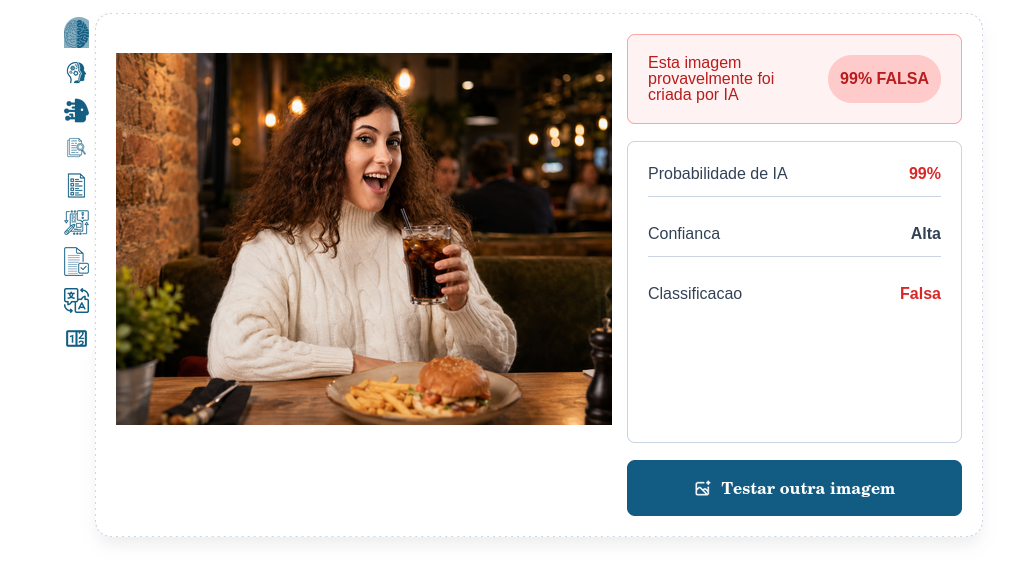
\includegraphics[width=0.48\textwidth]{../Exemplos/EditadaIA/TestePosTransformacao.png}
\hfill
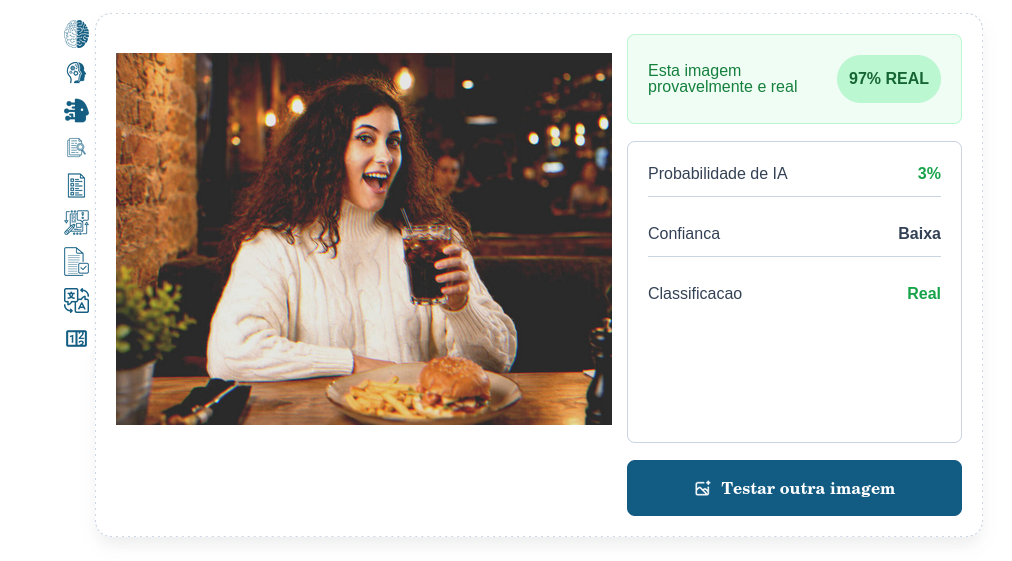
\includegraphics[width=0.48\textwidth]{../Exemplos/EditadaIA/TesteReducaoReso.png}
\caption{Resultados do ZeroGPT. À esquerda: fotografia real com cena transformada por IA ($\approx$99\% falsa). À direita: mesma imagem após compressão ($\approx$97\% real), evidenciando falha de detecção sob degradação digital.}
\label{fig:zerogpt-editada}
\end{figure}

A proposta metodológica adota o paradigma clássico de visão computacional --- extração de descritores manuais e classificação com SVM --- por alinhamento ao conteúdo da disciplina e por favorecer interpretabilidade quanto aos domínios de frequência, espaço e textura. Como base de dados, utilizar-se-á o CIFAKE, obtido de repositório público. Como complemento, caso haja disponibilidade, pretende-se analisar, de forma exploratória, como diferentes geradores contemporâneos produzem imagens, a fim de compreender ruídos e padrões associados e, potencialmente, aumentar a robustez da detecção.

%----------------------------------------------------------------------
\section{Trabalhos Relacionados}
%----------------------------------------------------------------------

A literatura de detecção de imagens sintéticas combina conjuntos de dados públicos, análise espectral, descritores handcrafted e métodos baseados em representações aprendidas.

Bird e Lotfi~\cite{bird2024cifake} introduziram o CIFAKE, composto por imagens reais do CIFAR-10 e imagens sintéticas geradas por Stable Diffusion, e reportaram acurácia próxima de 93\% com redes convolucionais. O CIFAKE constitui a base experimental desta proposta, por ser balanceado, documentado e já empregado em estudos de features manuais~\cite{nirob2026handcrafted}.

No domínio da frequência, Frank et al.~\cite{frank2020frequency} demonstraram que imagens produzidas por GANs exibem artefatos espectrais sistemáticos, associados a operações de \emph{upsampling}, o que permite separação eficiente e maior estabilidade perante perturbações como desfoque e recorte. Bammey~\cite{bammey2024synthbuster} estendeu a análise a modelos de difusão (Synthbuster), explorando picos no espectro de Fourier de um residual passa-alta e reportando detecção sob compressão JPEG leve. Tais resultados sustentam a inclusão de descritores espectrais e a avaliação sob JPEG neste trabalho.

Nirob et al.~\cite{nirob2026handcrafted} conduziram avaliação sistemática de descritores handcrafted (incluindo histograma de cores, DCT, HOG, LBP, GLCM e wavelets) sobre o CIFAKE, combinados a classificadores clássicos e a ensembles. A fusão de features apresentou desempenho competitivo, evidenciando a viabilidade de abordagens interpretáveis e computacionalmente leves --- alinhadas à escolha de FFT, HOG e LBP nesta proposta.

Choi et al.~\cite{choi2025warpad} apresentaram o WaRPAD, método \emph{training-free} que quantifica a sensibilidade de embeddings auto-supervisionados a perturbações em alta frequência relacionadas a crop/resize. Embora a arquitetura difira da adotada aqui, o trabalho reforça a hipótese de que transformações geométricas e de escala alteram indícios de síntese, o que motiva o protocolo experimental de robustez.

Em síntese, a literatura indica: (i)~utilidade de informação espectral e de textura~\cite{frank2020frequency,bammey2024synthbuster,nirob2026handcrafted}; (ii)~necessidade de avaliar transformações realistas~\cite{choi2025warpad,bammey2024synthbuster}. A lacuna explorada por esta proposta consiste em quantificar, sob o paradigma clássico (features + SVM) e sobre o CIFAKE, a degradação de desempenho por transformação e por família de descritores.

%----------------------------------------------------------------------
\section{Desenvolvimento}
%----------------------------------------------------------------------

Esta seção apresenta a versão prévia do plano metodológico: opções técnicas consideradas, justificativa das escolhas, dados e protocolo de avaliação.

\subsection{Objetivos e protocolo}

O protocolo experimental concentra-se na robustez a transformações: treinar o classificador exclusivamente em imagens intactas do CIFAKE e medir a variação de desempenho após transformações controladas, por família de feature. A Figura~\ref{fig:fluxo} resume o fluxo previsto, incluindo um laço de ajuste caso a robustez observada seja insuficiente.

\begin{figure}[ht]
\centering
\begin{tikzpicture}[
  node distance=0.55cm and 0.35cm,
  box/.style={draw, rounded corners, align=center, font=\footnotesize,
              inner sep=4pt, minimum width=2.8cm},
  dec/.style={draw, diamond, aspect=2.4, align=center, font=\scriptsize,
              inner sep=1pt},
  arr/.style={-{Latex}, thick}
]
  \node[box, fill=gray!15] (d) {CIFAKE\\real / fake};
  \node[box, below=of d] (f) {Extração FFT,\\HOG e LBP};
  \node[box, below=of f] (t) {Treinamento SVM\\(imagens intactas)};
  \node[box, below=of t] (x) {Transformações\\controladas};
  \node[box, below=of x] (e) {Avaliação por\\família de feature};
  \node[dec, below=0.65cm of e] (q) {Robustez\\suficiente?};
  \node[box, below left=0.75cm and 0.05cm of q, fill=green!12] (ok) {Análise e\\relato};
  \node[box, below right=0.75cm and 0.05cm of q, fill=orange!15] (aj) {Ajuste de\\descritores};

  \draw[arr] (d) -- (f);
  \draw[arr] (f) -- (t);
  \draw[arr] (t) -- (x);
  \draw[arr] (x) -- (e);
  \draw[arr] (e) -- (q);
  \draw[arr] (q) -- node[left, font=\scriptsize] {sim} (ok);
  \draw[arr] (q) -- node[right, font=\scriptsize] {não} (aj);
  \draw[arr] (aj.east) -- ++(0.5,0) |- (f.east);
\end{tikzpicture}
\caption{Fluxograma metodológico proposto sobre o CIFAKE: treinamento em imagens intactas, avaliação sob transformações e realimentação em caso de robustez insuficiente.}
\label{fig:fluxo}
\end{figure}

\subsection{Opções de técnicas e justificativa}

Foram consideradas três famílias de descritores, cobrindo os domínios usuais de processamento de imagens e com respaldo empírico na detecção de conteúdo sintético:

\begin{itemize}
\item \textbf{Frequência (FFT / espectro de magnitude):} motivada por artefatos de geração e pela sensibilidade da compressão JPEG ao conteúdo espectral~\cite{frank2020frequency,bammey2024synthbuster}.
\item \textbf{Espaço (HOG):} captura distribuição de gradientes e estrutura local, já empregada em avaliações handcrafted sobre o CIFAKE~\cite{nirob2026handcrafted}.
\item \textbf{Textura (LBP):} descreve padrões locais de intensidade; igualmente reportada como descritor competitivo em~\cite{nirob2026handcrafted}.
\end{itemize}

Como alternativas de classificação, contemplaram-se SVM, $k$-NN e ensembles (p.\ ex., LightGBM, conforme~\cite{nirob2026handcrafted}). Optou-se pelo \textbf{SVM} na etapa principal por: (i)~adequação a vetores de features de dimensão moderada; (ii)~uso consolidado em reconhecimento de padrões; (iii)~interpretabilidade relativa frente a redes profundas. Ensembles e $k$-NN permanecem como extensões opcionais para comparação.

Em relação a abordagens baseadas apenas em aprendizado profundo, priorizou-se a visão clássica nesta fase, tanto por alinhamento curricular quanto pela possibilidade de relacionar explicitamente a degradação observada a cada domínio de feature.

\subsection{Dados}

Utilizar-se-á o dataset CIFAKE~\cite{bird2024cifake}, também empregado por~\cite{nirob2026handcrafted}: aproximadamente 120\,000 imagens $32{\times}32$, balanceadas entre reais (CIFAR-10) e sintéticas (Stable Diffusion), com partição treino/teste. Os dados serão obtidos de repositório público (p.\ ex., Kaggle), sem coleta própria nesta etapa. Complementarmente, se houver condições, poderão ser inspecionadas amostras de geradores atuais (p.\ ex., ChatGPT/DALL$\cdot$E, Midjourney, Gemini/Nano Banana) apenas para caracterizar diferenças de geração e apoiar a robustez --- sem substituir o CIFAKE como base experimental.

A Figura~\ref{fig:zerogpt-editada} não integra o protocolo formal de métricas: serve apenas como motivação empírica do problema de robustez sob compressão.

\subsection{Transformações}

As transformações selecionadas simulam operações frequentes em redes sociais e pipelines de compartilhamento, em coerência com~\cite{bammey2024synthbuster,choi2025warpad}:

\begin{itemize}
\item compressão JPEG (fatores nominais 90\%, 70\% e 50\%);
\item geometria: redimensionamento e recorte (10\%, 25\% e 40\%);
\item filtragem: desfoque gaussiano (e, em extensão, nitidez/ajuste de brilho);
\item pipeline composto: recorte $\rightarrow$ redimensionamento $\rightarrow$ JPEG.
\end{itemize}

\subsection{Avaliação}

Reportar-se-ão acurácia e, quando pertinente, precisão e \emph{recall}, no conjunto de teste do CIFAKE sem transformação (\emph{baseline}) e após cada transformação, estratificando FFT, HOG e LBP. Espera-se identificar quais indícios visuais se degradam sob cada transformação e quais famílias de features apresentam maior estabilidade~\cite{frank2020frequency,nirob2026handcrafted,bammey2024synthbuster}.

\bibliographystyle{sbc}
\bibliography{referencias}

\end{document}
